%------------------------------------------------------------------------
%Editar Diplomado
\hypertarget{cv:GestionarProyectosColaboradores}{\section{Gestionar Proyectos de Colaborador}} \label{sec:GestionarProyectosColaboradores}

	Esta funcionalidad le permitirá las acciones necesarias para controlar los proyectos que han sido previamente registrados en el sistema de parte de líder de proyecto como lo es asignar colaboradores y gestionar los elementos que componen a un caso de uso..

		\subsection{Procedimiento}

			%Pasos de procedimiento
			\begin{enumerate}
	
			\item Seleccione la opción \textbf{Proyectos} del menú \ref{fig:MN-LP}.
	
			\item Se mostrará la pantalla \ref{fig:GestionarProyectosColaborador} ''Gestionar Proyectos de Colaborador''.

			\begin{figure}[htbp!]
				\begin{center}
					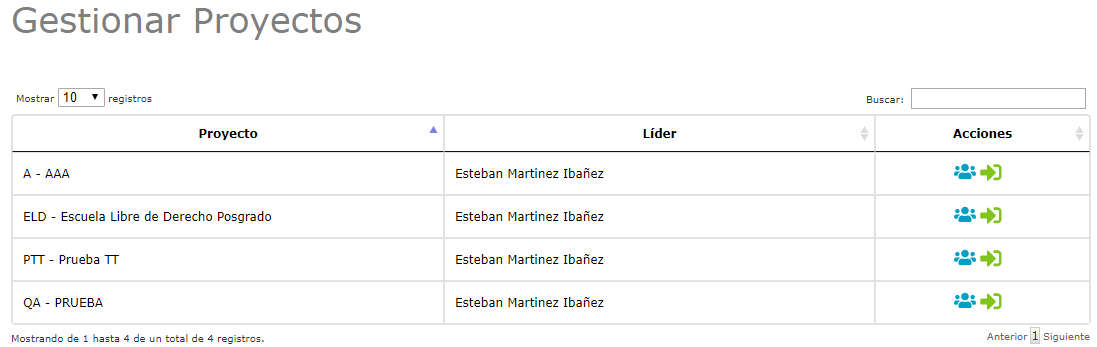
\includegraphics[scale=0.6]{roles/lider/proyectosColaborador/pantallas/IU4gestionarProyectosColaborador}
					\caption{Gestionar Proyectos de Colaborador}
					\label{fig:GestionarProyectosColaborador}
				\end{center}
			\end{figure}
		
				\item Seleccione la operación que desea realizar:
			
			Para (\hyperlink{cv:elegirColaboradores}{Elegir Colaboradores}) dé clic en el botón \IUAsignar.
			
			Para (\hyperlink{cv:DescargarDocumento}{Descargar Documento}) dé clic en el icono \IUPdf{} o \IUWord{} de algún proyecto ya registrado con elementos dentro del mismo.
			
			\end{enumerate}